\documentclass[12pt,titlepage]{article}
\usepackage{setspace}
\usepackage{fontspec}
\usepackage{pgfgantt}
\usepackage{multicol}
\usepackage{moreverb}
\usepackage{xcolor}
\usepackage{afterpage}
\usepackage{eso-pic}
\usepackage[figuresleft]{rotating}
\usepackage{url}
\def\UrlBreaks{\do\/\do-}
\usepackage
[
        a4paper,
        left=2.5cm,
        right=2.5cm,
        top=2.5cm,
        bottom=2.5cm
]
{geometry}
\setmainfont{Arial}
\pagenumbering{arabic}

\doublespacing
\usepackage{etoolbox}
\AtBeginEnvironment{quote}{\singlespacing\small}
\apptocmd{\thebibliography}{\raggedright}{}{}

\usepackage{natbib}
\newcommand*{\urlprefix}{Available at: }
\newcommand*{\urldateprefix}{Accessed }
\setcitestyle{notesep={: }}
\bibliographystyle{BCU.bst}

\immediate\write18{texcount -sum -1 \jobname.tex | xargs > \jobname.wc}
\newcommand\wordcount{\input{\jobname.wc}}

\definecolor{bbcnewsred}{RGB}{184,0,0}
\definecolor{bcublue}{RGB}{3,16,51}

\newcommand\NLStart[1]{\AtPageLowerLeft{%
\put(\LenToUnit{.505\paperwidth},\LenToUnit{.12\paperheight}){#1}%
}}%

\newcommand\BCUStart[1]{\AtPageLowerLeft{%
 \put(\LenToUnit{0\paperwidth},\LenToUnit{.12\paperheight}){#1}%
 }}%

\begin{document}

\begin{titlepage}
  \AddToShipoutPictureBG*{
    \BCUStart{\color{bcublue}\rule{.495\paperwidth}{.32\paperheight}}
    \NLStart{\color{bbcnewsred}\rule{.5\paperwidth}{.32\paperheight}}
  }
	\begin{center}
		\vspace*{1cm}

		\begingroup
      \fontsize{24}{30}\selectfont
      \textbf{BBC Feed}
    \endgroup

    \begingroup
      \fontsize{18}{22}\selectfont
      A Novel Interface for News Consumption Inspired by Social Media
    \endgroup

		\vspace{2cm}

		\textbf{Owen Tourlamain}

		\vfill

		Submitted in partial fulfilment of the requirements of Birmingham City University for the degree of Master of Science

		\vspace{0.8cm}

    \begin{multicols}{2}

      \color{white}

  		
\includegraphics[width=0.4\textwidth]{../img/bcu-logo.png}

  		%Computing, Engineering and the Built Environment\\
      CEBE\\
  		Birmingham City University\\
  		United Kingdom\\
      \columnbreak

      
\includegraphics[width=0.4\textwidth]{../img/nl-logo.png}

  		BBC News Labs\\
  		BBC\\
  		United Kingdom\\

    \end{multicols}

    \today - \wordcount words

	\end{center}
\end{titlepage}

\newgeometry{top=2.5cm,bottom=2.5cm,right=2.5cm,left=4cm}

\tableofcontents
\newpage

\section{Research Question}

How could social media delivery techniques be used in a digital news consumption platform to increase user engagement?

\section{Aims and Objectives}

  \subsection{Project Overview}

  This project aims to improve upon the flexibility and user engagement of
  traditional online news platforms, specifically those used by BBC News. The
  digital news landscape is changing rapidly; a report from Ofcom found that
  people in the UK are increasingly using digital platforms to consume news,
  often through the use of social media \cite{ofcom}. This project proposes that
  adapting user interface techniques from social media and applying them to a
  news app would help to keep users on the news platform. The system created
  will also aim to be flexible so that it can adapt to future changes in the
  digital news world.

  The project will be content-agnostic so that it can work with any future media
  that may be devised. To achieve this, the project will be divided into three
  parts: the feed, the catalogue and the scrapers. The feed will be an app that
  users can interact with. It will need to intelligently select content from the
  catalogue and present it to the user for consumption. The catalogue will store
  content that can be displayed, this will aim to be fast to access, and well
  organised to ensure a smooth flow of content to the users. The scrapers will
  create the content for the catalogue by connecting to various BBC news data
  sources. They will read this content, translate it into a form suitable for
  the catalogue and store it. Each one will have to be custom made for the
  various content sources.

  Social media often faces criticism for being addictive and of wasting users
  time \cite{neyman}. This raises ethical considerations with this project as it
  has the potential to also create these same issues. This should be mediated by
  the lack of user created content, meaning that the users time will be spent
  browsing informative news rather than wasting it. The addictive nature of
  social media is actually a benefit to this project as it is trying to
  increase user engagement on news platforms.

  \subsection{Key Terminology}

  \textbf{Infinite scrolling}: A user interface paradigm that presents content in a
  scrollable window. Before the end of the content is reached more content is
  loaded, resulting in the content appearing infinite to the user. This is often
  seen in social media, for example Facebook's newsfeed, and Twitter's timeline.

  \textbf{News Content}: For the purposes of this study news content will be
  defined as text, audio, photos or videos that are created or distributed by a
  news agency. These can come from a variety of sources ranging from broadcast
  news programmes to stock photos used within an article.

  \subsection{Deliverables and Goals}

  The deliverables for this project will be the three components highlighted
  above, as well as all documentation required to understand, maintain, deploy
  and use the system. The documentation will be provided as HTML pages alongside
  documentation within the codebase. The majority code produced will be written
  in Python.

    \subsubsection{The Feed}

    This deliverable will be a Python Flask application that can either be run
    locally or deployed to a web server. It will have accompanying scripts that
    install any pre-requisites for running the application. This deliverable
    will depend on having a valid catalogue to read from. If the hosted
    catalogue is unavailable there will be options to read from a local version.

    \subsubsection{The Catalogue}

    This deliverable will take the form of an SQL database schema. The database
    that it describes will be hosted on an AWS RDS instance. As this may not be
    available at all times the feed will have the ability to deploy a local
    database to read from for testing purposes.

    \subsubsection{The Scrapers}

    This part of the project consists of several independent scripts, each will
    be tailored to a specific BBC data source. The specifics for language,
    running and hosting will vary between the scripts. They will each come with
    appropriate documentation.

  \subsection{Out of Scope Issues}

  This project is primarily focused on the engineering challenges of developing
  this system, as such it will not be attempting to measure user experiences in
  any way. The project will also not be attempting to judge the performance of
  the content selection algorithm that is used. These topics are highly
  important to the problem space being explored, however they each could
  constitute a project in their own right and would spread the focus of this
  project too thin. These two issues would make for excellent follow up projects
  however so some comments may be made where relevant to future research.

\section{Background and Rationale}

  \subsection{Overview of the Problem Space}

  Modern news consumption started with the newspaper. Despite moving to online
  platforms these roots can still be seen in the user interfaces of digital news
  platforms such as the BBC News website and mobile app \cite{ofcom}. These
  interfaces broadly function by providing categories of content to browse, this
  makes these interfaces good for researching topics and for getting an overview
  of recent news within a topic \cite{yalanska_2021}. Social media instead often
  delivers content to users through an infinitely scrolling feed. This style of
  interface fits well with short bursts of interaction, such as while waiting
  for a kettle to boil or waiting for a bus \cite{yalanska_2020}. In these
  scenarios users often want to consume content without having to choose a
  category or risk running out of content.

  This style of interface removes the need for the end user to decide what
  content they consume at the point of consumption, instead they control what
  content is presented to them by following, liking, subscribing to or otherwise
  choosing to receive content from a number of sources. From this user input a
  social media platform will choose exactly which content to provide to a user,
  and in which order. The specifics of how these decisions are made are closely
  guarded secrets, and as such will not be investigated here.

  While social media allows users to access news content in this way, it is
  often preferential to deliver news to users on a first party platform, such as
  the app or website of the news agency. This gives the producers of the content
  more control over how it is presented and consumed, as well as what other
  content may be presented to the user alongside the current content. This
  project aims to create an interface inspired by social media, but completely
  controlled by the news agency.

  This also gives the creators of this content more flexibility to experiment
  with new content types, they are not limited to the narrow selection of media
  that the various social platforms offer. This feed can also offer features
  such as A/B testing that would enable the content producers to test the
  effectiveness of new media types \cite{ab}.

  When creating printed media, such as a newspaper, each article or photograph
  that is included takes up space that could have been used for something else.
  Because of this it is key to only select content that will have the greatest
  impact, and testing new content is risky. In an infinite scrolling style of
  interface however there is no limit on the amount of content that can be shown
  to a user, as such inserting new media forms to test them becomes more viable
  as if the user is not interested they can scroll past and move on to the next
  piece of content.

  \subsection{Motivation for the Project}

  This last issue is the primary inspiration for this project. As part of the
  BBC News Labs team I worked on the SlicerAV and Live Segment Notifications
  (LSN) projects. SlicerAV takes broadcast news programmes and automatically
  breaks them up into "slices" of short form media \cite{slicer}. Once this
  project was functional the next question was how to deliver this content to
  end users. For testing purposes we decided to tweet the slices as we felt that
  they fit best on to a social media platform, and twitter worked best for our
  use-case.

  The LSN project aimed to inspect news broadcasts just before they go live and
  notify users about upcoming content that may be interesting to them
  \cite{lsn}. This worked well, however we didn't have a good platform for
  hosting this content internally. This raised to possibility of a feed that
  would hold all the slices that a user had been notified about for them to
  browse. We then took that idea and realised it might fit well if applied to a
  news homepage, where sliced content could be surfaced alongside regular
  articles and videos.

  News Labs is focused on innovating news production and consumption, as such
  they have several projects that could benefit from a flexible user interface
  to surface their content. One such project is Graphical Story Telling (GST)
  which aims to take articles and turn them into a series of graphics with
  overlaid text that can be swiped through \cite{gst}. This content is inspired
  by social media and would fit perfectly into this project. This provided the
  idea to make a flexible feed that can present a wide variety of content in one
  place, with functionality for personalisation and testing.

\section{Literature Review}

  \subsection{Interfaces for Online News Consumption}

  Since the popularity of online news has taken off, there has been a lot of
  innovation and experimentation into the interfaces we use to consume this
  media. Most news agencies have tried to move away from simply displaying walls
  of text to users, in \cite{msnbc} we see a case study into how one large news
  agency re-designed their user interface, and the software stack that runs it.
  This study highlights how important flexibility was in the system, they split
  the system between the front end and the back end with the goal that "User
  interfaces and databases would become isolated components to be updated and
  swapped out" \cite{msnbc}. This closely mirrors the model proposed in this
  project. The case study also made note of the new system allowing content to
  reach audiences that hadn't been considered targets when the content was
  produced:

  \begin{quote}
    The same trading zone-style compromise also made it possible to take advantage
    of moments of alignment between editorial staffs and products whose tenor and
    target audiences might be viewed as incompatible on a larger scale.
  \end{quote}

  This shows that the connections to the SlicerAV project should prove useful,
  as that will allow segments of broadcast programmes to reach audiences that
  the whole programme may not.

  Some projects have taken this redesign in a different direction, in
  \cite{newsstand} we see an attempt to display news content based on it's
  geographical location. Localised news has always been popular, with the BBC
  running separate news programmes for different UK regions. This approach would
  allow a user to browse content purely by location which may have advantages to
  both end users and content producers. A map interface will not be a part of
  this project, however it is worth keeping in mind when building the data
  structures so that out of the box ideas like this can be built in the future.

  One key element to all major user interface redesigns is that they should be
  an improvement in some regard to the old system. Whether that is measured in
  loading speed, running costs, or any other metric, the improvement should be
  measurable in someway. Testing the proposed system against the current BBC
  News user interface would be a monumental task, requiring data that cannot be
  easily accessed. As such the measurement is out of scope for this project,
  however the means to perform those tests should be built into the system. In
  order to identify which metrics are important to track we can look at
  \cite{ux} and \cite{engagement}. \cite{ux} highlights that simple metrics,
  such as time spent browsing or number of articles viewed, are not sufficient
  on their own as both high and low figures for these can indicate good and bad
  user experiences. \cite{ux} found that the best way to measure user engagement
  was through interviews, this would be impractical to use all the time. Instead
  this project will aim to include some form of user feedback into the system,
  this will likely be modelled on a favourites system or a positive/negative
  indicator.

  \subsection{Infinite Scrolling User Interfaces}

  \cite{newtarget} defines infinite scrolling as:

  \begin{quote}
    a technique that allows users to scroll through a massive chunk of content
    with no finish line in sight. This technique simply keeps refreshing a page
    when you scroll down it.
  \end{quote}

  This description highlights how simple this design pattern is from a users
  point of view, but goes on to show how much of an impact it can have on the
  users. It states that users often feel that they "might be missing out on
  information" \cite{newtarget} as there is always more content being added to
  their screen. One possible solution it offers for this is some form of marker
  to show users how far they have gotten in the list and allow them to return
  later, this will be considered as a feature for this project.

  \cite{neyman} and \cite{karlsson} have looked into the negatives of infinite
  scrolling interfaces, highlighting the addictive nature and that users often
  waste time while using them. For the purposes of this project however these
  features are actually helpful as there is a desire to increase engagement on
  the BBC News platforms, and the users time will not be wasted as they will be
  browsing informative and well written news articles. Both studies do however
  note that too much choice can be a bad thing, \cite{karlsson} states:

  \begin{quote}
    while people may be attracted by a large variety of options, they are more
    likely to act when given fewer choices.
  \end{quote}

  This is something to keep in mind when designing this system, we should aim to
  not overload the user with too many options at once. Techniques such as
  allowing users to save articles for later, return to their position in the
  list and allowing them to filter content to different categories will help to
  overcome this.

  Another aspect to consider is the implementation, as mentioned by
  \cite{newtarget} infinite scrolling has the potential to reduce the
  responsiveness of the interface as more content is loaded. \cite{tajima} used
  SuperSQL in order to work around some of these issues, this may be a fitting
  technique for this project as it will be using a relational database. As a lot
  of content will have to be loaded, small delays between system components will
  quickly add up resulting in a poor user experience. To combat this each
  element of the system will need to be tested thoroughly and UI tasks such as
  rendering should be separated from other logic through threading.

  \subsection{Social Media Design for Increasing User Engagement}

  Social media is not a new concept to news distribution. \cite{standley} found
  in a survey that social media is now the most commonly used communication
  channel on the internet. \cite{boukes} found that social media ranked highly
  as an important source for news, especially among younger audiences. This has
  naturally caused many news outlets to start publishing content on social
  media, this however has not come without any downsides. \cite{boukes} showed
  that "Twitter usage positively influenced knowledge acquisition [and] Facebook
  had a negative effect", they suggest that this is corelated to the target
  users of the platforms, stating that twitter users are often motivated to use
  the platform to gain knowledge and information. This means that using these
  techniques on a news app or website should work well, as the audience will have
  visited the service with the purpose of gaining information.

  This project has one key difference from social media, in that it will not
  contain any user made content. \cite{zhang} found that an infinite feed
  increased appreciation of content produced by others, but decreased users
  desire to create their own content. Since there will be no ability to create
  user content this will not be an issue for this project.

  There are a lot of negative effects often associated with social media. As
  this project is taking inspiration from this area it is worth taking steps to
  ensure that these negatives are not a part of this new system.
  \cite{lupinacci} suggests that a lot of these issues stem from a state of
  "continuous connectedness" to other people. Users will not be connected to
  each other in this system, however they may still experience these issues by
  being constantly connected to the world through the news. The best way to
  avoid this is a topic for a study in it's own right, for this project it is
  sufficient to be aware of the issue if it appears.

\section{Methodology and Planning}

  \subsection{Development Methodology}

  The development of this project will follow a Kanban-style methodology
  \cite{kanban}. Since there is only one developer on this project this will not
  be used for collaborative purposes, instead it will be used to manage and
  monitor tasks. As tasks arise they will be added to a To-Do list. These will
  me moved to an In Progress list when they are started and then a Done list
  when finished. Tasks will be added, edited and split into subtasks as needed
  throughout the project. This methodology will allow a high degree of
  flexibility which fits the project well as the specifics of the project will
  likely evolve as the project progresses.

  \subsection{Project Timeline}

  Time management for this project will be monitored through the use of a Gantt
  chart (see fig. \ref{fig:gantt}). Contingency time has not yet been added to
  the plan, this will be added after development has started when project pacing
  can be measured. This chart will be updated as the project develops, however
  more granular tasks will not be added. These will be tracked through the
  Kanban board mentioned in the methodology.

  \clearpage

  \begin{sidewaysfigure}
    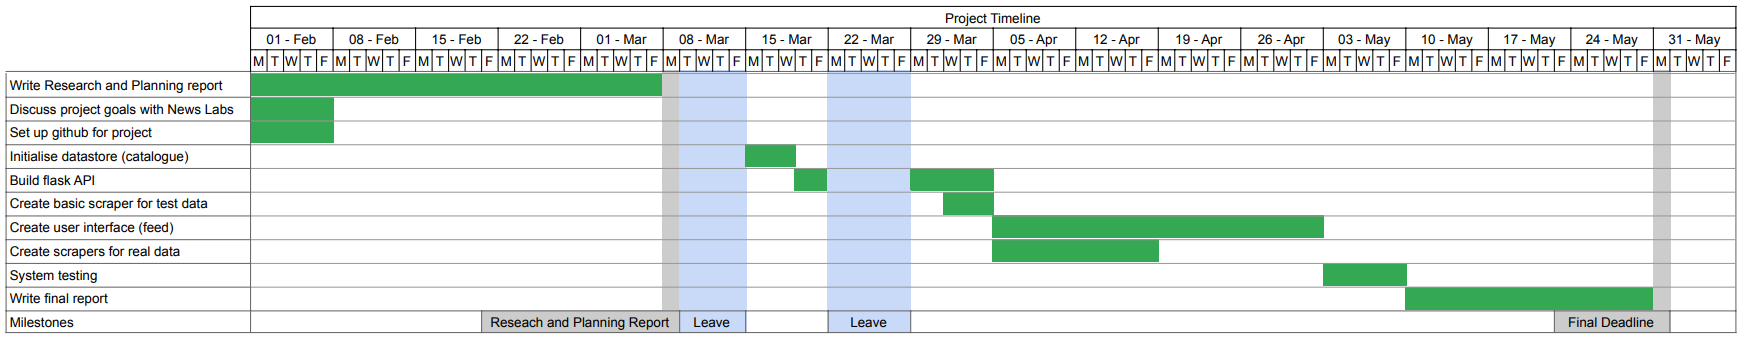
\includegraphics[width=\textheight]{../img/gantt.png}
    \caption{Project timeline gantt chart}
    \label{fig:gantt}
  \end{sidewaysfigure}

  \clearpage

\bibliography{research_and_planning}

\end{document}
